\documentclass[a4paper]{article}

\usepackage{Sweave}
\begin{document}
\Sconcordance{concordance:r-sveave-example.tex:r-sveave-example.Rnw:%
1 2 1 1 0 6 1 1 2 1 0 1 1 9 0 1 2 5 1 2 2 2 1}


R Sveave example:
In this example we embed parts of the examples from the
\texttt{kruskal.test} help page into a LaTeX document:

\begin{Schunk}
\begin{Sinput}
> data (airquality)
> kruskal.test(Ozone ~ Month, data = airquality)
\end{Sinput}
\begin{Soutput}
	Kruskal-Wallis rank sum test

data:  Ozone by Month
Kruskal-Wallis chi-squared = 29.267, df = 4, p-value = 6.901e-06
\end{Soutput}
\end{Schunk}

which shows that the location parameter of the Ozone
distribution varies significantly from month to month.
Finally we include a boxplot of the data:

\begin{center}
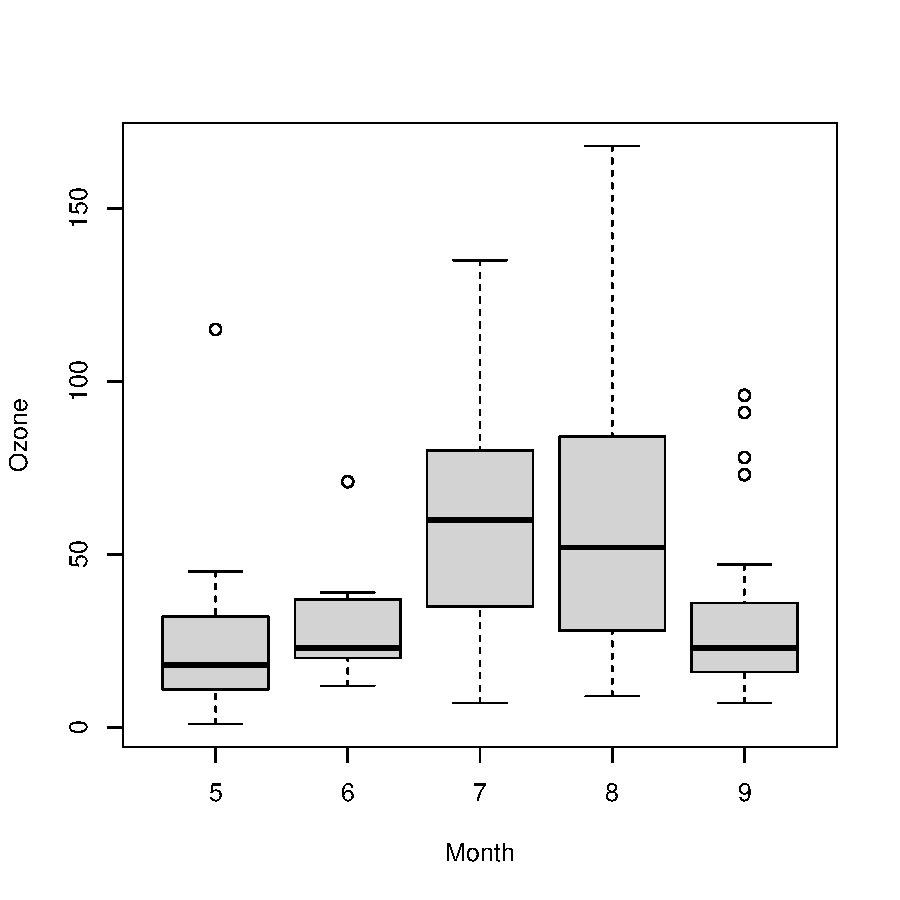
\includegraphics{r-sveave-example-002}
\end{center}

\end{document}
